\documentclass[12pt]{article}
\usepackage[margin=1in]{geometry}
\usepackage{graphicx}
\usepackage{setspace}
\usepackage{url}

\title{Tecellate: A Distributed Environment for Ad Hoc Wireless Network Simulations}
\author{
        Steve Johnson (srj15@case.edu)\\
        Case Western Reserve University\\
        \and Tim Henderson (tah35@case.edu)\\
        Case Western Reserve University
}
\date{\today}

\begin{document}
\doublespacing
\maketitle

% \begin{multicols}{2}

\begin{abstract}
    Tecellate is a simulation which autonomous agents can move in a grid and communicate using
    semi-realistic radio signals. The simulation itself can be distributed over multiple machines to
    allow for very large simulations. The system allows researchers to test various wireless network
    protocols and algorithms under arbitrarily harsh conditions.
    
    The usefulness of the simulation was tested using an approximated IP stack. Our initial results
    show that the simulation produces useful information, though more work is required to improve
    its accuracy.
\end{abstract}

\section{Introduction}

Computer network modeling and simulation has become an important tool in the arsenal of any computer
networks researcher. It has only become more important as increasingly research into mobile
and autonomous devices matures. Large scale simulations of thousands to hundreds of thousands of
devices become increasingly crucial to validate techniques without having to spend thousands of
dollars on costly equipment. To support such simulations we present Tecellate, a horizontally
scalable distributed network simulator.

Tecellate simulates the physical layer of the network. All \textbf{agents} (actors in the
simulation) have a ``radio'' to send and receive byte strings. To approximate the real world, these
byte strings may be probabilistically corrupted as a function of distance and interference. To
provide reliable communication between arbitrary agents, users must implement the link, IP, and
transport layers. As a resource to users wishing to model the traditional TCP/IP stack the authors
provide a partial implementation up to the IP layer.\footnote{
  We hope to expand this implementation to include the TCP and UDP transport layers as well.
}

In the physical world, devices move around with purpose and transmit with purpose. We assert that
the same should be true in a simulation. However, modeling the purpose of actual people is not
possible. Therefore, the simulation gives the agents an alternative purpose: to stay alive. Each
agent has to ``eat'' in order to survive. Each turn, each agent may eat a unit of food if its
current location contains food. If it runs out of food, it dies. The goal of the agents is to stay
alive as long as possible. Thus, it must find sources of food within the simulation. This game-like
element provides the agents with goals and a purpose for communication.

As wireless networks become more widespread, the number of participants in a given network will
grow. Simulations that are not scalable may become too slow to simulate important test cases. For
this reason, Tecellate is designed to scale horizontally across many machines.

By modeling the communication at the physical layer and adding game-like elements to our simulation,
we hope to provide an interesting test bed for networking and AI algorithms. The game-like element
in our simulation will help ensure the agents move around purposefully in the simulation grid. The
physical layer simulation ensures that the communication problems which must be overcome for
reliable communication are similar to real world problems. The inherent scalability of the system
should allow simulation of arbitrarily large scenarios. While, we do not think our simulation
approach would be the final word in networks simulation, it should provide a useful platform for
experimentation.

\section{Literature Survey}

There are a few existing simulations of wireless ad hoc networks that operate above the link layer.
One of these is ns2, which has been around for several years \cite{ns2}. ns2 simulates multiple
kinds of networks and protocols, and it has been popular among researchers. However, it is difficult
to scale above a few hundred nodes \cite{swans}. It has only been documented to scale to a few
thousand nodes.

GloMoSim is a newer simulator \cite{glomosim}. It serves a similar purpose to ns2 and can simulate
both wired and wireless networks, but it is more scalable in that it can run its event loop in
parallel \cite{swans}. It can scale to tens of thousands of nodes.

SWANS is a simulator created purely for ad hoc wireless network research in response to the
inadequacy of ns2 and GloMoSim for ad hoc wireless network research \cite{swans}. It has a different
configuration/modeling style from other solutions which allows it to accurately simulate millions of
nodes on 2004 hardware.

A specialized wireless ad hoc network simulator is $madhoc$, a system that attempts to accurately
model wireless network characteristics in metropolitan settings \cite{madhoc}. The authors argue
that other simulators' node movement algorithms do not accurately model real world environments, and
consequently spend a great deal of effort modeling the characteristics of metropolitan environments.

These simulators differ from Tecellate in that they simulate a higher level of the network and
provide no inherent goal for communicating agents. They also simulate radio signal propagation much
more accurately, which affects the computation requirements drastically. They have sophisticated
physics-based models of signal strength which must be updated and accounted for when sending and
receiving transmissions, while we propose to use simpler probabilistic methods at the bit level.


\section{Simulation Rules} \label{rules}

The simulation runs in discrete steps (\textbf{turns}). The conceptual ``length'' of a turn is
designed to simulate the time to send $k$ bytes, where $k$ is a configurable constant. Each turn, an agent may do any combination of the following: listen, broadcast, move, or die.

\subsection{Movement}

The simulation world consists of a $w$*$h$ grid of signed integers. If a cell's value $c$ is
non-negative, it is the terrain height. Otherwise, the cell is impassable. An agent can move at most
one cell up, down, left, or right per turn. However, after moving into a square, it must wait $c$
turns before it may make another move.

An agent's move may succeed or fail. If an agent tries to move into an impassible cell, it will
fail. It will also fail if it tries to move into a cell that was occupied by another agent at the
end of the last turn, \textbf{or} a cell that another agent attemps to move into in the same turn.
These cases are shown in figure \ref{mvt}.

\begin{figure*}[h!]
    \begin{center}
        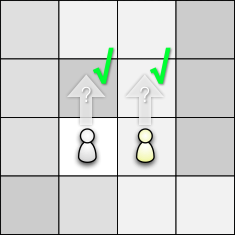
\includegraphics[width=1in]{figures/mvt1.png}
        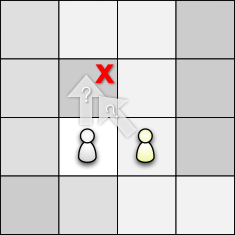
\includegraphics[width=1in]{figures/mvt2.png}
        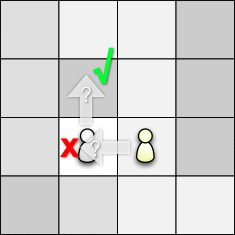
\includegraphics[width=1in]{figures/mvt3.png}
    \end{center}
    \caption{Three main cases for movement.}
    \label{mvt}
\end{figure*}

It may seem more intuitive for both moves in case 3 to succeed, i.e. a move $Z\rightarrow Y$ should
succeed if agent $A$ moves $X\rightarrow Y$. However, allowing this case would introduce large
dependency graphs that would span a large geographical area. This kind of dependency graph would
greatly reduce the effectiveness of our horizontal scaling scheme based on geographical partitioning
described later in this paper.

\subsection{Messages}

The broadcast messages agents can send are a simpilification of radio communication. There are $N$
frequencies an agent can broadcast on or listen too. An agent may broadcast a message of 1024 bytes
on a single frequency. The agent may also listen for messages on $M$ frequencies each turn where $M
\leq N$.

Like radio communication, the messages broadcast decay over distance. When an agent listens to a
frequency, the agent always recieves data. However, if no one is broadcasting on that frequency, the
agent will recieve random data. Since the message decays over distance, even if an agent hears it
some parts of the message may be corrupted. The farther away a listener is from a sender, the more
corruption is in the message.

Finally, if more than one message can be heard from the same position, the messages will be combined
probabilistically.

% Finally, if messages cross each other the following algorithm will be used to resolve the
% conflict. First, for each message the message will be corrupted based on its distance to its source,
% just as in the single broadcaster senario. Then, for each bit in each message their will be a
% probability K that the bit will be heard. The probablity will also be based on the distance to the
% source of the message. All of the bits that are heard are XORed together creating a composite
% message. If not bit are heard for a particular bit location a random value is chosen for that bit.

\subsection{Perception}

Agents may or may not be informed of their global position in the world. They also have some way of
``seeing'' nearby agents.

\subsection{Food}

Agents must search the grid to find food. If their coordinator calculates that their food counter is
below zero, they disappear from the grid.

\section{Usefulness of the Simulation}

The simulation provides a close enough approximation of the real world to allow testing of
high-level coordination algorithms to be tested using a very simple API.

The rules for movement (1 delayed turn per cell height difference) and perception provide an
opportunity to experiment with pathfinding algorithms in an environment where little information
outside a limited area is available, similar to the conditions of the DARPA autonomous vehicle
events.

The rules for communication force agents to communicate with distant agents by passing messages
through nearby agents, creating ad-hoc wireless networks. Our messaging system is meant to model the
difficulties of real world radio communication. This will make our simulation a useful tool for
simulating adhoc wireless networks allowing protocol research to be conducted without hardware.


\section{Current State of the Project}

The simulation contains \textbf{agents} which must be sent stimuli to respond to. The current implementation consists of a \textbf{master process} which connects to several \textbf{coordinator processes} that are responsible for keeping the state of disjoint sets of agent processes.

The master process is responsible for connecting to the coordinators, sending them configurations, and waiting for their final responses. The coordinator connects to neighbor coordinators and agents, serves requests for information about the state of its agents in the last turn, and processes its own agents by requesting information from its neighbors and from its agents. In this way, the coordinators operate in lock-step, turn by turn, until all turns have been processed by all coordinators.

The current version of the simulation only supports agent movement and agent death. Agents are killed when they both occupy the same cell. The master process and coordinators do not attempt to balance load after the simulation has begun.


\section{Distributing Work}

Part of this project will include dynamically balancing the load of communication between agents and coordinators. There are at least three possible approaches to this problem in the context of this simulation.

The simplest way to assign agents to coordinators is to assign a constant number of agents to each agent coordinator at random or based on some positioning heuristic. No agents will ever change their coordinators. This strategy would create significant overhead from passing messages between agents on separate coordinators.

A more efficient strategy would be to assign each coordinator a section of the grid and have coordinators hand off responsibility for agents at the borders between coordinators. This way, coordinators would only need to exchange agent messages when the agents are near coordinator borders. One downside of this strategy is that some coordinators may be responsible for many more agents than others if agents cluster in a few areas.

This problem could be solved by allowing the master process to dynamically reallocate the space assigned to each coordinator. \textbf{This dynamic reassignment is very similar to the problem of assigning many application instances to many servers,} but in addition to simply trying to distribute CPU and memory load evenly, we are also trying to reduce the traffic between servers which must pass data to each other (agent broadcasts) for the simulation to be correct.


\section{Validation}

iaweofiaw efoaw iefj



\section{Conclusion}

This project has three layers. At the top layer, we want to refine a system that distributes work among several servers. At the middle layer, we want to implement a simulation. At the bottom layer, we want to use it as a testbed for ad-hoc wireless networks. For these reasons, we think it is a compelling course project.


\nocite{*}
\bibliographystyle{acm}
\bibliography{bibliography}

\end{document}
